\section{Примеры атаки}

\subsection{ARP-spoofing}

До выполнения ARP-spoofing'а в ARP-таблице узлов \textbf{A} и \textbf{B} существуют записи с IP- и MAC-адресами друг друга. Обмен информацией производится непосредственно между узлами \textbf{A} и \textbf{B}. (зелёная стрелка)

В ходе выполнения ARP-spoofing'а компьютер \textbf{C}, выполняющий атаку, отправляет ARP-ответы (без получения запросов):

\begin{itemize}
	\item узлу \textbf{A}: с IP-адресом узла \textbf{B} и MAC-адресом узла \textbf{C};
	\item узлу \textbf{B}: с IP-адресом узла \textbf{A} и MAC-адресом узла \textbf{C}.
\end{itemize}

\begin{figure}[H]
	\centering
	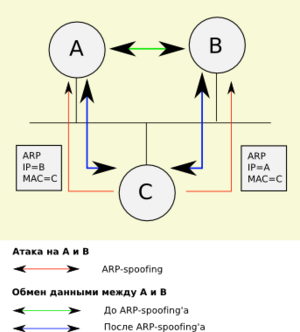
\includegraphics{img/arp-spoofing.png}
	\caption{ARP-spoofing}
\end{figure}

В силу того что компьютеры поддерживают самопроизвольный ARP (gratuitous ARP), они модифицируют собственные ARP-таблицы и помещают туда записи, где вместо настоящих MAC-адресов компьютеров \textbf{A} и \textbf{B} стоит MAC-адрес компьютера C. (красные стрелки)

После того как атака выполнена, когда компьютер \textbf{A} хочет передать пакет компьютеру \textbf{B}, он находит в ARP-таблице запись (она соответствует компьютеру \textbf{C}) и определяет из неё MAC-адрес получателя. Отправленный по этому MAC-адресу пакет приходит компьютеру \textbf{C} вместо получателя. Компьютер \textbf{C} затем ретранслирует пакет тому, кому он действительно адресован — т.е. компьютеру \textbf{B}. (синие стрелки)


\subsection{DHCP-spoofing}

Несмотря на то, что DHCP является протоколом прикладного уровня модели OSI, основная его работа сосредоточена на канальном уровне. Это означает, что возникновение проблем с его функционированием будет иметь последствия на одном из самых базовых уровней сети.

Первое сообщение DHCP Discover от клиента \textbf{Host} является широковещательным, то есть его получат все пользователи сети, в том числе сервер \textbf{DHCP\_server} и злоумышленник \textbf{Rogue}. Они отправят свои ответы DHCP Offer клиенту, из которых он должен выбрать то, что его «устроит». По умолчанию в большинстве систем клиент выбирает первое пришедшее предложение, игнорируя остальные. Таким образом, открывается брешь: если ответ от \textbf{Rogue} придёт раньше, атака окажется успешной. Сервер может быть физически более удалён от клиента, чем злоумышленник, а также быть менее быстрым, поэтому вероятность успешной реализации атаки довольно высока.

\begin{figure}[H]
	\centering
	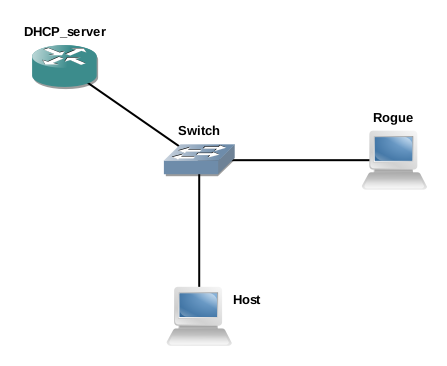
\includegraphics{img/dhcp.png}
	\caption{DHCP-spoofing}
\end{figure}


Последствия:

\begin{itemize}
	\item Злоумышленник может в своём ответе клиенту указать неправильные данные о сети, что приведёт к невозможности его дальнейшей работы, то есть будет реализован отказ в обслуживании.
	\item В большинстве случаев протокол DHCP предоставляет клиенту информацию о шлюзе по умолчанию. Таким образом, злоумышленник имеет возможность указать себя в качестве шлюза, что является реализацией атаки <<человек посередине>> на сетевом уровне.
\end{itemize}

